\documentclass{beamer}

\usepackage{graphics}
\usepackage{listings}
\usepackage{verbatim}

\usetheme{Berlin}
\usecolortheme{albatross}

\title{Einstein on a Computer}
\author{Joey Bernard - ACEnet CRC}
\date{November 2010}

\begin{document}
\maketitle

\begin{frame}
  \frametitle{What we'll cover}
  A look at computational science
  \begin{itemize}
    \item What is General Relativity?
    \item Why is it hard?
    \item Finding a solution - techniques
    \item Using Einstein Toolkit
  \end{itemize}
\end{frame}

\begin{frame}
  \frametitle{What is General Relativity?}
  \begin{itemize}
    \item Developed by Einstein between 1907 - 1915
    \item Accounted for problems in Newtonian theory
    \begin{itemize}
      \item the precession of the orbit of Mercury
      \item bending of star light around the sun
      \item progression of time differing in different gravitational fields
    \end{itemize}
  \end{itemize}
\end{frame}

\begin{frame}
  \frametitle{General Relativity - 2}
  A couple of the key ideas of General Relativity
  \begin{itemize}
    \item time is just another dimension, treated the same as the three spatial dimensions
    \item the speed of light, c, is the absolute speed limit locally
    \item acceleration and gravitation are indistinguishable
    \item gravitational force comes from bent spacetime
    \item spacetime bends due to mass and energy
  \end{itemize}
\end{frame}

\begin{frame}
  \frametitle{Why is it hard?}
  \begin{LARGE}
  \begin{center}
    $ \textbf{G} = \frac{8 \pi G}{c^4} \textbf{T} $
  \end{center}
  \end{LARGE}
  \begin{itemize}
    \item \textbf{G} - tensor describing spacetime geometry
    \item \textbf{T} - tensor describing mass-energy
    \item G - gravitational constant
    \item c - speed of light
  \end{itemize}
\end{frame}

\begin{frame}
  \frametitle{Hard - 2}
  \begin{LARGE}
  \begin{center}
    $ G_{\mu \nu} + \Lambda g_{\mu \nu} = \frac{8 \pi G}{c^4} T_{\mu \nu} $
  \end{center}
  \end{LARGE}
  \begin{itemize}
    \item  $\Lambda$ is the cosmological constant (Einstein's biggest mistake that likely wasn't a mistake)
    \item The $\mu$ and $\nu$ are indices for the tensors
    \item Indices run through 1 for each dimension (e.g. 3+1)
    \item This means that for regular 4-dimensional spacetime, we end up with a system of 10 coupled, nonlinear, hyperbolic-elliptic PDEs
  \end{itemize}
\end{frame}

\begin{frame}
  \frametitle{Hard - 3}
  Only the simplest solutions have an exact solution
  \begin{itemize}
    \item Schwarzschild (1915-1916) - Completely empty space with a single point source of mass (static, spherically symmetric)
    \item Reissner-Nordstrom (1916-1918) - static, spherically symmetric, charged
    \item Kerr (1963) - rotating, spherically symmetric
    \item Kerr-Newman (1965) - rotating, spherically symmetric, charged 
  \end{itemize}
  These lead to various black hole solutions. \\
  Anything more realistic needs a numeric solution.
\end{frame}

\begin{frame}
  \frametitle{Finding a solution - techniques}
  Basic technique breaks down into two separate problems
  \begin{itemize}
    \item initial value problem
    \item evolution problem
  \end{itemize}
  Useful for
  \begin{itemize}
    \item cosmological models
    \item critical phenomena
    \item perturbed black holes / neutron stars
    \item coalescence
  \end{itemize}
\end{frame}

\begin{frame}
  \frametitle{Solutions 2}
  Break down spacetime back into 3+1 dimensions
  \begin{itemize}
    \item a set of 3-dimensional hypersurfaces, separated across time
    \item a lapse function describing how to go from one hypersurface to another
    \item a shift function describing how points on the hypersurfaces move around, from one hypersurface to another
  \end{itemize}
\end{frame}

\begin{frame}
  \frametitle{Solutions 3}
  \begin{itemize}
    \item Begin with a snapshot of the gravitational fields on some hypersurface (initial data)
    \item Evolve this data to the next hypersurface
    \item Like all numerical analysis, need to pay attention to stability and convergence
    \item Need to pay attention to the following to produce accurate solutions
    \begin{itemize}
      \item gauge conditions
      \item coordinates
      \item actual formulation of the Einstein equations
    \end{itemize}
  \end{itemize}
\end{frame}

\begin{frame}
  \frametitle{Solutions 4}
  \begin{itemize}
    \item Richard Arnowitt, Stanley Deser, Charles W. Misner - first published in the late 1950's
    \item The ADM formalism, decomposes spacetime into 3 space and 1 time dimensions
    \item Almost nobody uses the original ADM formulation, but most modern formulations are based on this
    \item First recorded attempt was Hahn and Lindquist in 1964
    \item Limited to 2+1 dimensions (cylindrical symmetry)
  \end{itemize} 
\end{frame}

\begin{frame}
  \frametitle{Solutions 5}
  Timeline of computational work:
  \begin{itemize}
    \item Early 1980's - gravitational waveforms from formation of a rotating black hole
    \item Late 1990's - head-on binary black hole collision
    \item 1995 - first 3D solution of a Schwarzschild black hole
    \item 1990's - introduction of excision and puncture methods to deal with singularities
    \item 1990's - adaptive mesh refinement introduced from computational fluid dynamics
    \item 2005 - first publication of merger of two black holes through excision
  \end{itemize}
\end{frame}

\begin{frame}
  \frametitle{Using Einstein Toolkit}
  \begin{itemize}
    \item Cactus Code is a software framework for high-performance computing
    \item Structured as a core portion (called the flesh), and plugins (called thorns)
    \item Plugins for Cactus Code include things like IO, scientific file formats, evolution engines, etc.
    \item Einstein Toolkit spun off as a separate project to focus on solving Einstein's equations 
  \end{itemize}
\end{frame}

\begin{frame}
  \frametitle{Einstein 2}
  \begin{itemize}
    \item 1995 - Cactus Code developed at the Max Planck Institute, version 1 released
    \item 1999 - Version 4.0 Beta 1 released
    \item 2003 - Several members of the group left Germany to help found the Center for Computation and Technology at Louisiana State University. Development now happening at both sites
    \item Feb. 2009 - Version 4.0 Beta 16 released
    \item 2010 - Einstein Toolkit has first release
  \end{itemize}
\end{frame}

\begin{frame}
  \frametitle{Einstein 3}
  \begin{itemize}
    \item The flesh is independent of the thorns and provides the main program which parses the parameters and starts up the appropriate thorns
    \item No actual work is done by the flesh
    \item All user-supplied code goes into thorns
    \item Thorns are essentially independent, they communicate through the flesh API
  \end{itemize}
\end{frame}

\begin{frame}
  \frametitle{Einstein 4}
  \begin{itemize}
    \item Connections between thorns and flesh are handled through configuration files
    \item These are parsed at compile time
    \item Glue code is generated to encapsulate the external appearance of the thorn
    \item Mostly calls to registration routines in the flesh
    \item At runtime, the executable reads a parameter file that says which thorns should be activated, with what parameters
  \end{itemize}
\end{frame}

\begin{frame}
  \frametitle{Einstein 5}
  Thorns specific to the Einstein toolkit
  \begin{itemize}
    \item time evolution methods
    \item initial data generators
    \item file readers
  \end{itemize}
  This provides a common set of tools for numerical relativity that you can extend and build on.
\end{frame}

\begin{frame}
  \frametitle{Einstein 6}
  \begin{itemize}
    \item The central thorn is ADMBase, provides
    \begin{itemize}
      \item standard set of variables (metric, lapse, shift, curvature)
      \item these are used for data import and export
      \item not necessarily good for evolution
    \end{itemize}
    \item Other thorns have the responsibility to translate these variables into their required form
    \item This allows different thorns to have access to the same data
  \end{itemize}
\end{frame}

\begin{frame}
  \frametitle{Einstein 7}
  Einstein-Hydrodynamics Coupling
  \begin{itemize}
    \item Everything up till now has been vacuum
    \item There are thorns to provide matter fields
    \item TmunuBase has a standard set of variables and a set of schedule groups orchestrating when $T_{\mu\nu}$ is calculated
  \end{itemize}
\end{frame}

\begin{frame}
  \frametitle{Example - Grazing black holes}
  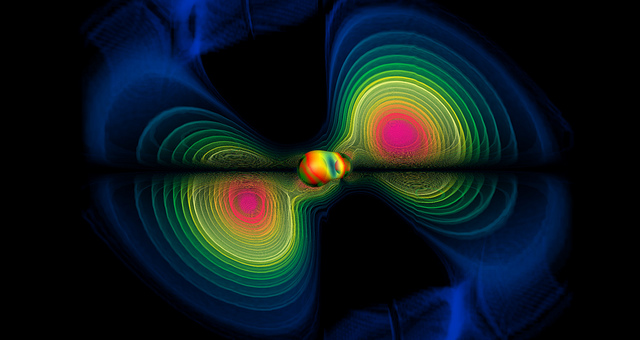
\includegraphics[scale=0.5]{image1.jpg}
\end{frame}

\begin{frame}
  \frametitle{Example - Binary waves}
  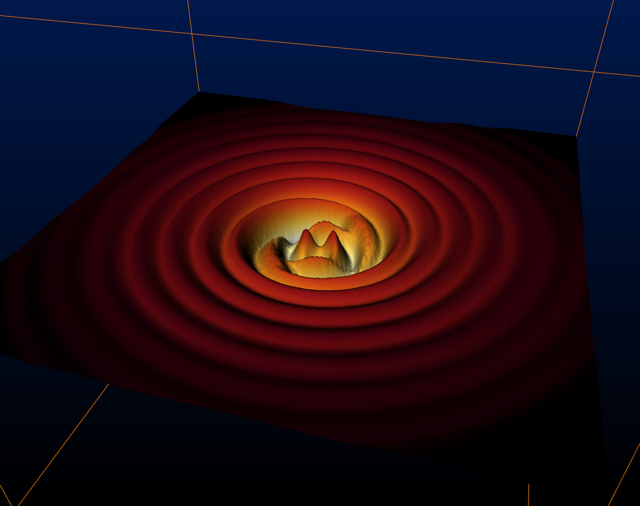
\includegraphics[scale=0.5]{image2.jpg}
\end{frame}

\begin{frame}
  \frametitle{What's the point to me?}
  \begin{itemize}
    \item Fundamental physics
    \item Electron-positron collision
    \item The resulting gamma rays
    \item Do they mesh? If not, what's wrong?
  \end{itemize}
\end{frame}

\end{document}

